% Created 2020-11-04 Wed 09:52
% Intended LaTeX compiler: pdflatex
\documentclass[presentation]{beamer}
\usepackage[utf8]{inputenc}
\usepackage[T1]{fontenc}
\usepackage{graphicx}
\usepackage{grffile}
\usepackage{longtable}
\usepackage{wrapfig}
\usepackage{rotating}
\usepackage[normalem]{ulem}
\usepackage{amsmath}
\usepackage{textcomp}
\usepackage{amssymb}
\usepackage{capt-of}
\usepackage{hyperref}
\usetheme{UoB}
\author{Mark Blyth}
\date{\textit{[2020-11-02 Mon]}}
\title{Knots, collocation, writing}
\hypersetup{
 pdfauthor={Mark Blyth},
 pdftitle={Knots, collocation, writing},
 pdfkeywords={},
 pdfsubject={},
 pdfcreator={Emacs 27.1 (Org mode 9.3)}, 
 pdflang={English}}
\begin{document}

\maketitle

\section{Background}
\label{sec:org742cc8f}
\begin{frame}[label={sec:org6695432}]{Week's activities}
\begin{itemize}
\item Spline-Newton CBC with more knots
\begin{itemize}
\item Goal: more numerical stability
\item Different results, but not really any better
\end{itemize}
\end{itemize}
\vfill
\begin{itemize}
\item Looked into collocation references
\end{itemize}
\vfill
\begin{itemize}
\item Started annual review report
\end{itemize}
\end{frame}

\section{More-knots CBC}
\label{sec:orgee4e00c}
\begin{frame}[label={sec:org18b7fbc}]{Newton iteration issues}
\begin{itemize}
\item Converged solution doesn't actually solve continuation equations
\begin{itemize}
\item Newton iterations should, but don't, give a vector that, when passed to the continuation equations, give a zero output
\item More iterations don't help
\item Different convergence criteria don't improve things
\end{itemize}
\end{itemize}
\vfill
\begin{itemize}
\item Solution jumps
\begin{itemize}
\item Jacobian is always well-conditioned
\item Probably a finite-differences issue?
\end{itemize}
\end{itemize}
\vfill
\begin{itemize}
\item Idea: try more knots!
\begin{itemize}
\item More knots = more attainable accuracy = perhaps better chance of finding a solution
\end{itemize}
\end{itemize}
\end{frame}

\begin{frame}[label={sec:orgc29e5cb},plain]{Baseline: 5 knots}
\begin{center}
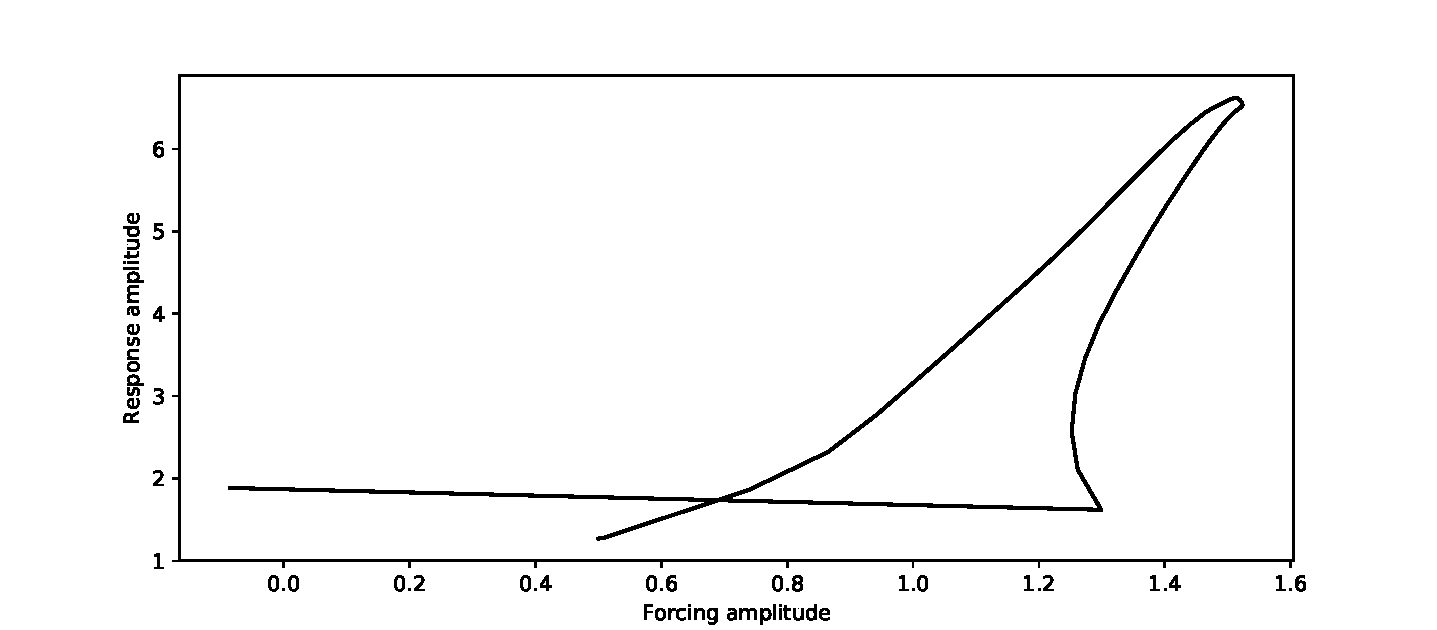
\includegraphics[width=.9\linewidth]{./5_knots_cbc.pdf}
\end{center}

\begin{itemize}
\item Minimum 3 interior knots for a valid BSpline model
\item Solution jumps
\item Converged Newton-iteration vectors don't solve the continuation equations accurately
\end{itemize}
\end{frame}

\begin{frame}[label={sec:org9235877},plain]{20 knots}
\begin{center}
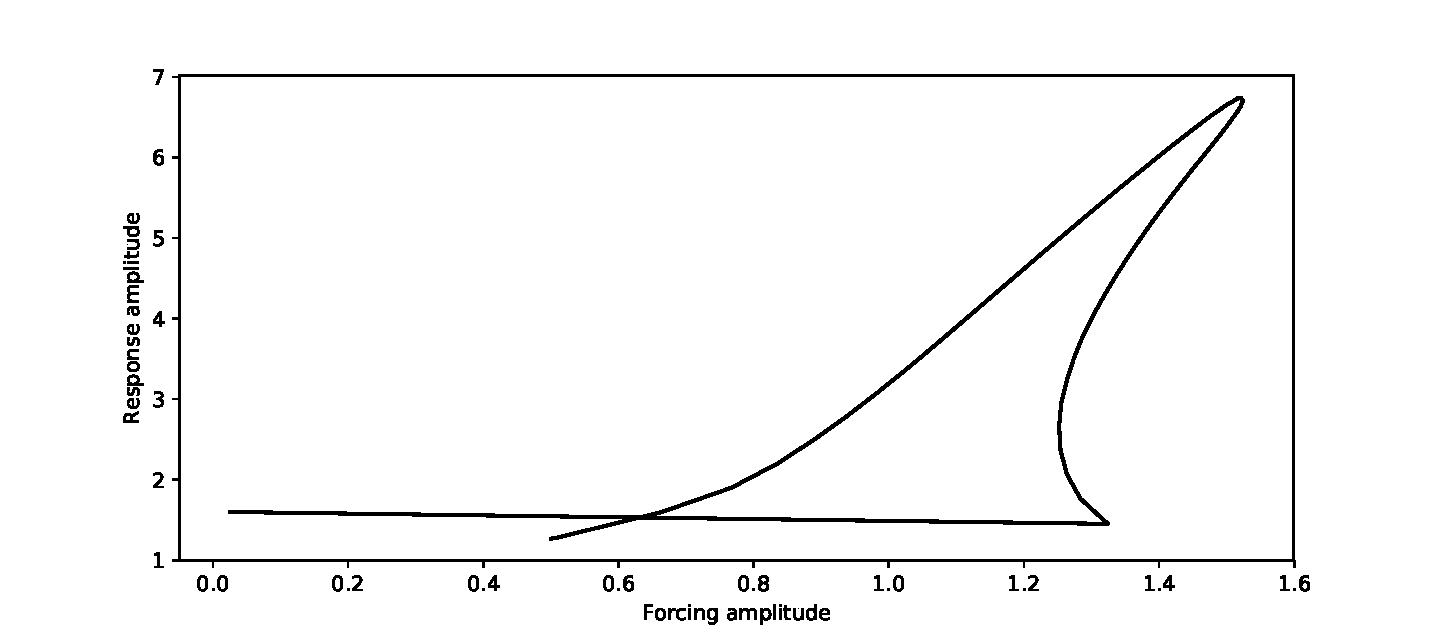
\includegraphics[width=.9\linewidth]{./20_knots_cbc.pdf}
\end{center}

\begin{itemize}
\item Simulation is notably slower to run
\item Solution still jumps
\item Converged Newton-iteration vectors solve system to higher accuracy than before
\end{itemize}
\end{frame}

\begin{frame}[label={sec:org88cf10b},plain]{30 knots}
\begin{center}
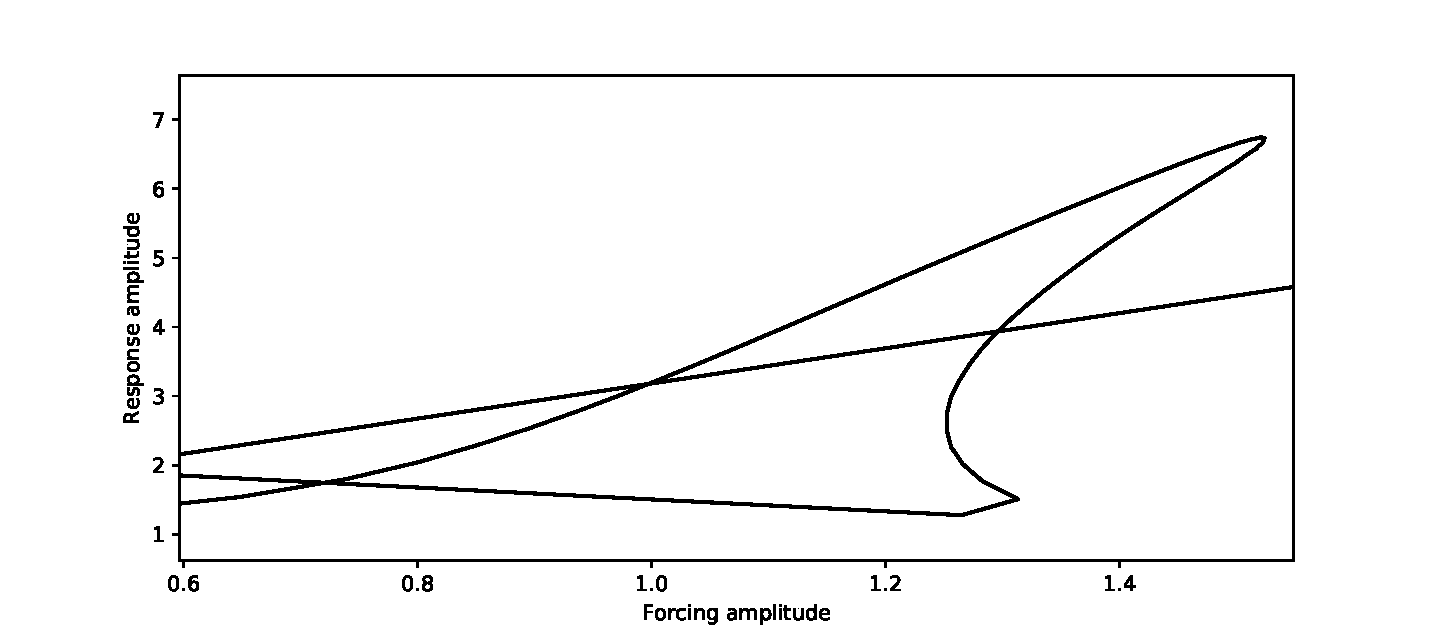
\includegraphics[width=.9\linewidth]{./30_knots_zoom.pdf}
\end{center}

\begin{itemize}
\item Simulation is even slower to run
\item Solution jumps at about the same place
\item Converged Newton-iteration vectors again solve system to higher accuracy
\end{itemize}
\end{frame}

\begin{frame}[label={sec:org6113814}]{Things to note}
\begin{itemize}
\item SciPy solvers still get a solution with 5 knots
\begin{itemize}
\item Means the equations can be solved, but not by the Newton solver
\item Presumably then, finite differences is unable to find an accurate gradient?
\end{itemize}
\end{itemize}

\vfill
\begin{itemize}
\item Solution is jumping after the second fold
\begin{itemize}
\item I'd have expected this to be one of the more numerically stable places
\end{itemize}
\end{itemize}
\end{frame}

\begin{frame}[label={sec:org9b8f27f}]{Other things to try}
\begin{itemize}
\item Adaptive stepsize
\begin{itemize}
\item Should allow greater accuracy around difficult regions (eg. folds)
\end{itemize}
\end{itemize}
\vfill
\begin{itemize}
\item Adaptive knots
\begin{itemize}
\item Essential for `harder' (eg. neuronal) signals
\item (Presumably) unimportant here
\end{itemize}
\end{itemize}
\vfill
\begin{itemize}
\item Idea: Jacobian checking
\begin{itemize}
\item Use a secant predictor to estimate the next Jacobian
\item If the finite-differences Jacobian differs much from the secant prediction, try FD again with a new stepsize
\item Extension: adaptive-stepsize finite differences
\end{itemize}
\end{itemize}
\end{frame}

\section{New gain CBC}
\label{sec:org8930d19}
\begin{frame}[label={sec:org1e39b62}]{Effects of control gain}
Another thing to try: increasing the control gain
\vfill
\begin{itemize}
\item Was originally using \(K_p = 1\)
\begin{itemize}
\item This worked fine for Duffing Fourier
\item Keeping \(K_p\) as low as possible seems to give the best-possible accuracy with Fourier
\end{itemize}
\end{itemize}
\vfill
\begin{itemize}
\item Intuitively, increasing \(K_p\) would make it \emph{harder} to find a correct solution, not easier
\begin{itemize}
\item Smaller gains mean bigger proportional errors mean more difference between invasive and noninvasive targets, between solutions and non-solutions
\item In limit, large \(K_p\) means every control target solves the continuation equations, whether or not they're noninvasive
\item Intuition: smaller \(K_p\) gives a larger gradient at the fixed-point, and therefore a more accurate solution can be found
\end{itemize}
\end{itemize}
\end{frame}

\begin{frame}[label={sec:org860db2f},plain]{5 knots, \(K_p = 2\)}
\begin{center}
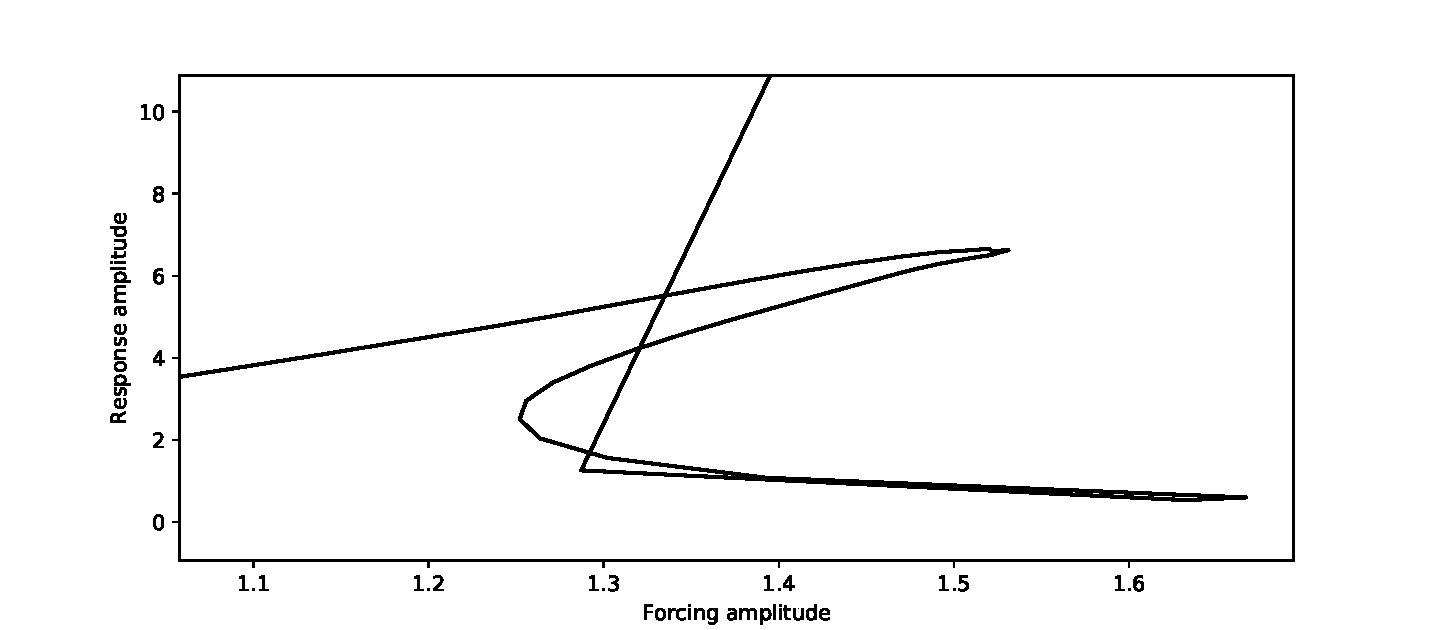
\includegraphics[width=.9\linewidth]{./5_knots_cbc_kp_2.pdf}
\end{center}

\begin{itemize}
\item Unexpected: slight improvement in results
\item Using \(K_p = 2\) delayed the `jump'
\begin{itemize}
\item Jump region is controllable with \(Kp=1\) for Fourier, but not splines
\end{itemize}
\item \alert{Still doesn't explain why non-Newton solvers could find a solution at \(K_p=1\)!}
\begin{itemize}
\item If the SciPy solver can find a solution at \(K_p = 1\), why can't a Newton solver?
\end{itemize}
\end{itemize}
\vfill
Idea: what's the solution basin of attraction?
\end{frame}

\begin{frame}[label={sec:org727a869},plain]{20 knots, \(K_p = 2\)}
\begin{center}
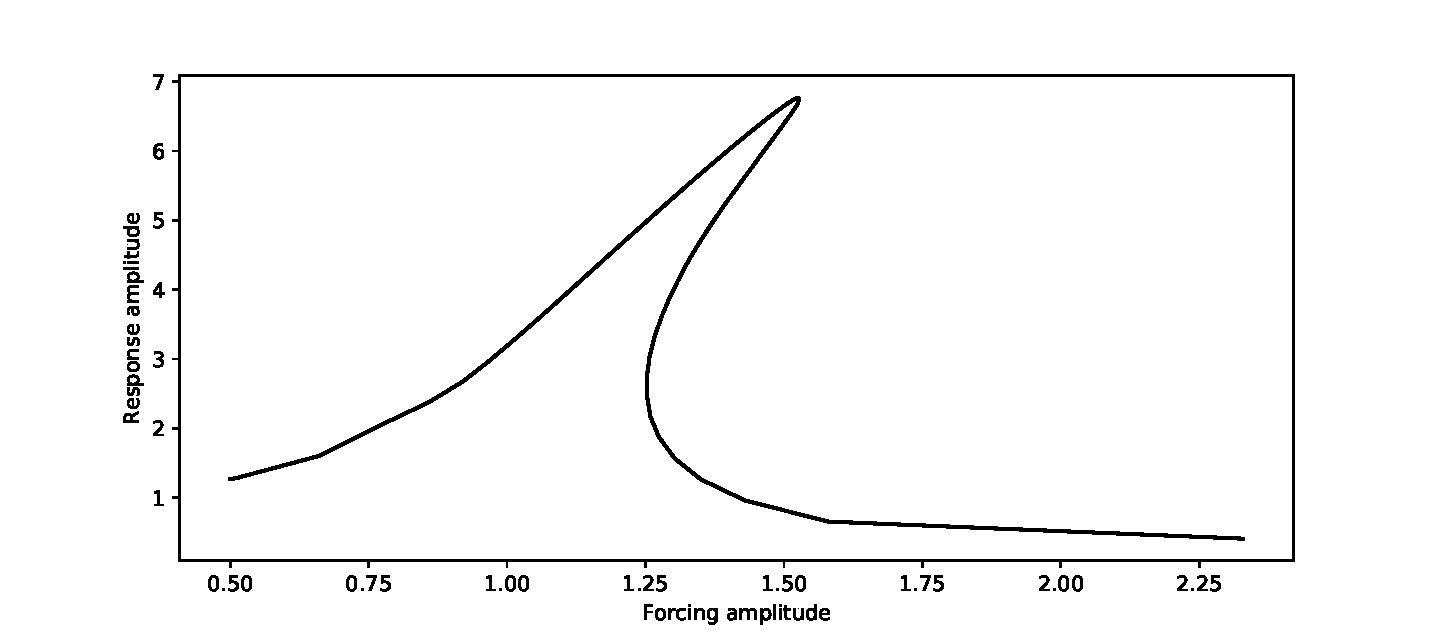
\includegraphics[width=.9\linewidth]{./20_knots_kp_2.pdf}
\end{center}

\begin{itemize}
\item Solution takes a huge leap at the end, but it's a correct leap
\item It works, but doesn't seem like it should; opposite result to what was expected
\item \alert{Still doesn't explain what was going wrong with \(K_p = 1\)}
\end{itemize}
\end{frame}

\section{Collocation}
\label{sec:org7b0cb54}
\begin{frame}[label={sec:orgbb6050d}]{Standard continuation}
Other work: considering a `standard' (non-control-based) continuation of the Duffing oscillator
\vfill
\begin{itemize}
\item Removes any issue from controllers being weird
\item Simplifies down to just a discretisation and predictor/corrector problem
\end{itemize}
\vfill
\begin{itemize}
\item Plan of action:
\begin{enumerate}
\item Learn about collocation and periodic-orbit continuation \alert{\emph{[in progress]}}
\item Learn about BSpline collocation for BVPs \alert{\emph{[in progress]}}
\item Combine them
\item Add in the extras (BSpline periodicity structure, choice of knots, choice of collocation meshpoints, if any)
\item Code up and test
\item Make the step 4 extras adaptive
\end{enumerate}
\end{itemize}
\end{frame}

\section{Next steps}
\label{sec:org6338b8c}
\begin{frame}[label={sec:orgba86097}]{Next steps}
\begin{itemize}
\item Annual review report
\end{itemize}
\vfill
\begin{itemize}
\item Then\ldots{}
\begin{itemize}
\item More collocation
\item `Standard' continuation
\item Investigate solution basin of attraction?
\item Adaptive CBC algos
\end{itemize}
\end{itemize}
\end{frame}
\end{document}
